%%%%%%%%%%%%%%%%%%%%%%%%%%%%%%%%%%%%%%%%%%%%%%%%%%%%%%%%%%%%%%%%%%%%%%%%%%%%%%%
%% SOCIOL 723 -- Social Statistics II
%% Week 10 -- Panel Data and Difference-in-Differences
%% Wenhao Jiang, Duke University, Fall 2026
%%%%%%%%%%%%%%%%%%%%%%%%%%%%%%%%%%%%%%%%%%%%%%%%%%%%%%%%%%%%%%%%%%%%%%%%%%%%%%%

\documentclass[aspectratio=169,11pt,xcolor=dvipsnames]{beamer}
\mode<presentation>

%% ---- fonts: Latin Modern Roman (the LaTeX default), serif throughout -------
\usepackage[T1]{fontenc}
\usepackage{lmodern}
\usefonttheme{serif}
\renewcommand{\familydefault}{\rmdefault}

%% ---- packages --------------------------------------------------------------
\usepackage{amsmath,amsfonts,amssymb,bm}
\usepackage{graphicx}
\usepackage{booktabs}
\usepackage{tikz}
\usetikzlibrary{arrows.meta,positioning,calc}
\usepackage[english]{babel}

\newcommand{\srcp}[1]{{\scriptsize\color{gray}(#1)}}
\newcommand{\srct}[1]{#1}

\DeclareMathOperator*{\argminop}{arg\,min}
\DeclareMathOperator*{\argmaxop}{arg\,max}
%% \limits forces the subscript underneath even in inline math
\newcommand{\argmin}{\argminop\limits}
\newcommand{\argmax}{\argmaxop\limits}
\DeclareMathOperator{\Cov}{Cov}
\DeclareMathOperator{\Var}{Var}
\DeclareMathOperator{\trace}{tr}
\DeclareMathOperator{\rank}{rank}
\DeclareMathOperator{\plim}{plim}
\newcommand{\indep}{\perp\!\!\!\perp}

%% ---- notation conventions (course-wide) ------------------------------------
\newcommand{\E}{E}
\newcommand{\En}{\mathbb{E}_n}
\newcommand{\R}{\mathbb{R}}
\newcommand{\X}{\bm{X}}
\newcommand{\Y}{\bm{y}}
\newcommand{\Ix}{\bm{I}}
\newcommand{\zero}{\bm{0}}
\newcommand{\bhat}{\hat{\bm{\beta}}}
\newcommand{\dto}{\overset{d}{\longrightarrow}}
\newcommand{\pto}{\overset{p}{\longrightarrow}}
\usetikzlibrary{shapes,decorations.pathmorphing}
\newcommand{\lik}{\mathcal{L}}
\newcommand{\loglik}{\ell}
\newcommand{\Info}{\mathcal{I}}
\newcommand{\SE}{\mathrm{se}}

%% ---- theme -----------------------------------------------------------------
\usetheme{default}
%% thin single-line header: clickable section names, current one highlighted.
%% (miniframes is deliberately not used: one dot per slide wraps to 4 rows here)
\setbeamerfont{section in head/foot}{size=\tiny}
\setbeamertemplate{headline}{%
  \begin{beamercolorbox}[wd=\paperwidth,ht=2.4ex,dp=1.1ex,%
                         leftskip=.3cm,rightskip=.3cm]{section in head/foot}%
    \usebeamerfont{section in head/foot}%
    \insertsectionnavigationhorizontal{.94\paperwidth}{}{}%
  \end{beamercolorbox}%
}

\definecolor{dukeblue}{RGB}{1,33,105}
\definecolor{accent}{RGB}{200,78,0}
\definecolor{softgray}{RGB}{242,242,245}

\setbeamercolor{structure}{fg=dukeblue}
\setbeamercolor{frametitle}{fg=dukeblue,bg=white}
\setbeamercolor{section in head/foot}{fg=white,bg=dukeblue}
\setbeamercolor{section in head/foot shaded}{fg=white!50!dukeblue,bg=dukeblue}
\setbeamercolor{alerted text}{fg=accent}
\setbeamercolor{block title}{fg=white,bg=dukeblue}
\setbeamercolor{block body}{fg=black,bg=softgray}
\setbeamercolor{block title alerted}{fg=white,bg=accent}
\setbeamercolor{block body alerted}{fg=black,bg=softgray}

\setbeamertemplate{footline}[page number]
\setbeamertemplate{navigation symbols}{}
%% continued frames keep the SAME font size and spill onto a new slide
\setbeamertemplate{frametitle continuation}{\ifnum\insertcontinuationcount>1\normalfont\footnotesize\ (cont.)\fi}
\setbeamertemplate{itemize items}[circle]
\setbeamertemplate{blocks}[rounded][shadow=false]
\setbeamerfont{frametitle}{series=\bfseries}
\setbeamerfont{footnote}{size=\scriptsize}
\setbeamerfont{caption}{size=\footnotesize}
\setbeamertemplate{subsection in head/foot}{}
\setbeamertemplate{subsection in head/foot shaded}{}
\setbeamertemplate{caption}[numbered]

\newcommand{\adv}{\,\raisebox{0.6pt}{\textcolor{accent}{$\bigstar$}}}
%% marker for essential material every student must understand (examinable core)
\definecolor{corestar}{RGB}{0,83,155}
\newcommand{\core}{\,\raisebox{0.6pt}{\textcolor{corestar}{$\bigstar$}}}

\setbeamertemplate{section page}{%
  \begin{centering}\vfill
  {\usebeamercolor[fg]{structure}\Large\bfseries\insertsectionhead\par}
  \vskip4pt{\color{dukeblue}\rule{0.35\linewidth}{1pt}\par}
  \vfill\end{centering}}
\setbeamertemplate{subsection page}{%
  \begin{centering}\vfill
  {\usebeamercolor[fg]{structure}\large\bfseries\insertsubsectionhead\par}
  \vfill\end{centering}}

\AtBeginDocument{%
  \setlength{\abovedisplayskip}{5pt}%
  \setlength{\belowdisplayskip}{5pt}%
  \setlength{\abovedisplayshortskip}{2pt}%
  \setlength{\belowdisplayshortskip}{3pt}%
}
\setbeamertemplate{frametitle}{%
  \vskip4pt\usebeamerfont{frametitle}\usebeamercolor[fg]{frametitle}%
  \insertframetitle\par\vskip2pt}
\setbeamersize{text margin left=0.75cm, text margin right=0.75cm}

%% ---- title -----------------------------------------------------------------
%% ---- title page: same face as the body (Latin Modern), larger and bold
\setbeamerfont{title}{size*={16}{19},series=\bfseries}
\setbeamerfont{subtitle}{size=\Large,series=\mdseries}
\setbeamerfont{author}{size=\large}
\setbeamerfont{date}{size=\large}
\title[SOCIOL 723]{SOCIOL 723: Social Statistics II\\[-2pt]}
\subtitle{Week 10, Panel Data and Difference-in-Differences\\[-6pt]}
\author[Jiang]{Wenhao Jiang\vspace{-2.5em}}
\institute[Duke]{}
\titlegraphic{
\includegraphics[height=1.3cm]{../Misc/duke_logo.png}}
\date{Department of Sociology, Fall 2026}


\begin{document}

\begin{frame}[plain]
  \titlepage
\end{frame}

\begin{frame}{Today}
  \tableofcontents
  \vskip6pt
  {\footnotesize \core{} $=$ essential, you must understand this \quad\quad \adv{} $=$ for understanding, not examined}
\end{frame}

\begin{frame}{A Third Source of Variation}
So far: adjust for observables (Week 6), find an instrument (Week 7), find a
threshold (Week 9). Today: use \alert{variation over time within the same unit}.
\vskip4pt
\begin{block}{The core idea}
If we observe the same unit before and after, we can difference away everything
about that unit that does not change, including confounders we never measured
and could not name.
\end{block}
\vskip4pt
\begin{itemize}\itemsep2pt
  \item That is a genuinely powerful trick, and it is why panel data are prized.
  \item It buys nothing against confounders that \emph{do} change over time, and
        the price is a new and demanding assumption about counterfactual trends.
  \item The last decade has shown that the standard implementation, 
        two-way fixed effects, is badly behaved in exactly the setting
        sociologists use most.
\end{itemize}
\end{frame}

%%%%%%%%%%%%%%%%%%%%%%%%%%%%%%%%%%%%%%%%%%%%%%%%%%%%%%%%%%%%%%%%%%%%%%%%%%%%%%%
\section[Panel Data]{Panel Data and Unobserved Heterogeneity}
%%%%%%%%%%%%%%%%%%%%%%%%%%%%%%%%%%%%%%%%%%%%%%%%%%%%%%%%%%%%%%%%%%%%%%%%%%%%%%%
\begin{frame}\sectionpage\end{frame}

\begin{frame}{The Error Components Model\core}
With unit $i$ observed at times $t = 1,\dots,T$:
\begin{align*}
  Y_{it} = \beta D_{it} + \underbrace{\alpha_i}_{\text{unit effect}}
         + \underbrace{\lambda_t}_{\text{time effect}} + \epsilon_{it} .
\end{align*}
\vskip3pt
\begin{itemize}\itemsep3pt
  \item $\alpha_i$ absorbs \emph{every} time-invariant characteristic of unit $i$
, observed or not, nameable or not.
  \item Pooled OLS is biased whenever $\Cov(D_{it},\alpha_i)\neq 0$: states that
        adopt a policy differ persistently from states that do not.
  \item \textbf{Random effects} assumes $\Cov(D_{it},\alpha_i)=0$ and is more
        efficient if true. It is almost never true in the settings we care about.
        The Hausman test compares the two; when in doubt, use fixed effects.
\end{itemize}
\end{frame}


\begin{frame}[allowframebreaks,t]{The Within Transformation, Explicitly\core}
Average the model within unit and subtract:
\begin{align*}
  Y_{it} &= \beta D_{it} + \alpha_i + \lambda_t + \epsilon_{it} \\
  \bar Y_{i\cdot} &= \beta \bar D_{i\cdot} + \alpha_i + \bar\lambda + \bar\epsilon_{i\cdot} \\[2pt]
  \Longrightarrow\quad
  Y_{it} - \bar Y_{i\cdot} &= \beta\big(D_{it}-\bar D_{i\cdot}\big)
  + (\lambda_t - \bar\lambda) + \big(\epsilon_{it}-\bar\epsilon_{i\cdot}\big) .
\end{align*}
\vskip3pt
\begin{itemize}\itemsep3pt
  \item $\alpha_i$ is gone, \alert{whatever it was}. That is the whole appeal:
        we never had to name it, measure it, or model it.
  \item Anything time-invariant is annihilated with it. You cannot estimate the
        effect of race, sex, or birth cohort in a unit-fixed-effects model, not
        because they do not matter but because there is no within-unit variation.
  \item Two-way fixed effects demeans within unit \emph{and} within period,
        removing common shocks.
  \item The equivalence with unit dummies is \alert{exactly FWL from Week 1}:
        regressing on unit dummies partials out the unit means.
\end{itemize}
\end{frame}

\begin{frame}[allowframebreaks,t]{Random Effects, and Why We Usually Do Not Use It}
Random effects treats $\alpha_i$ as a draw from a distribution and assumes the
unit effect is unrelated to the regressors. The slogan version is
$\Cov(D_{it}, \alpha_i) = 0$, but consistency needs the stronger statement
\begin{align*}
  \E\big[\alpha_i \mid D_{i1},\dots,D_{iT}\big] = 0 ,
\end{align*}
mean independence from the \emph{whole history} of the regressor, together with
strict exogeneity of the idiosyncratic error, $\E[\epsilon_{it}\mid D_{i1},\dots,D_{iT},\alpha_i]=0$.
It then estimates by GLS, a matrix-weighted average of the within and between
estimators.
\vskip3pt
\begin{itemize}\itemsep3pt
  \item \textbf{If the assumption holds}, RE is more efficient and can identify
        coefficients on time-invariant covariates. That is a real gain.
  \item \textbf{The assumption says states that adopt a policy are, on average,
        no different from states that do not.} In the settings sociologists study
        it is almost never plausible.
  \item The \textbf{Hausman test} compares the two: a large difference indicates
        $\Cov(D,\alpha)\neq 0$ and favours FE. But failing to reject is weak
        evidence, as usual.
  \item \alert{The default should be fixed effects}, with random effects reserved
        for cases where you can defend the exogeneity of the unit effect, or
        where the multilevel structure is itself the object of interest.
\end{itemize}
\end{frame}

\begin{frame}[allowframebreaks,t]{Nickell Bias and the FE-versus-LDV Choice}
Sociologists routinely control for last year's outcome, to absorb differences
between units that are \emph{changing} rather than fixed. It is a reasonable
instinct. But combining that move with unit fixed effects creates a new bias, and
it is worth knowing why before you reach for it.
\vskip3pt
Add a lagged dependent variable to a fixed-effects model:
\begin{align*}
  Y_{it} = \rho Y_{i,t-1} + \beta D_{it} + \alpha_i + \epsilon_{it} .
\end{align*}
Demeaning makes $Y_{i,t-1} - \bar Y_{i\cdot}$ mechanically correlated with
$\epsilon_{it} - \bar\epsilon_{i\cdot}$, because $\bar Y_{i\cdot}$ contains
$Y_{it}$, which contains $\epsilon_{it}$.
\vskip3pt
\begin{itemize}\itemsep2pt
  \item The resulting \alert{Nickell bias} is $O(1/T)$: severe in short panels
        ($T = 3$), negligible in long ones. Arellano--Bond-type GMM instruments
        the lagged difference with deeper lags.
  \item \textbf{FE and LDV embody different selection stories}: FE assumes
        selection on time-invariant traits; LDV assumes selection on prior
        outcomes. They can both be valid, but they are different assumptions and
        will generally give different answers.
  \item \srct{Angrist and Pischke (2009)} suggest running both: under some
        conditions the two \alert{bracket} the truth, so agreement is reassuring
        and disagreement tells you how much the selection story matters. Treat
        that as a heuristic, not a theorem.
\end{itemize}
\end{frame}

\begin{frame}{Three Ways to Remove $\alpha_i$}
\begin{center}\small
\renewcommand{\arraystretch}{1.5}
\begin{tabular}{lll}
\toprule
Estimator & Transformation & Note \\
\midrule
Within (fixed effects) & $Y_{it}-\bar Y_i = \beta(D_{it}-\bar D_i) + \tilde\epsilon_{it}$
  & the default \\
First difference & $\Delta Y_{it} = \beta \Delta D_{it} + \Delta\epsilon_{it}$
  & equals within when $T = 2$ \\
Unit dummies & include $n-1$ indicators & numerically identical to within \\
\bottomrule
\end{tabular}
\end{center}
\vskip5pt
\begin{itemize}\itemsep2pt
  \item All three remove $\alpha_i$; the first two are transformations, the
        third does it with parameters. The costs (previous frames) are shared.
  \item Within and first differences differ when $T > 2$ and disagree under
        serial correlation; report which you used and why.
\end{itemize}
\end{frame}

\begin{frame}{What Fixed Effects Costs\core}
\begin{itemize}\itemsep3pt
  \item \textbf{Precision}. You are using only within-unit variation. If $D_{it}$
        barely moves within units, the standard error explodes, FWL again.
  \item \textbf{Measurement error is amplified}. Differencing removes signal and
        keeps noise, so attenuation bias gets worse.
  \item \textbf{Nickell bias and the FE-versus-LDV choice}, as on the previous
        frames: adding a lagged outcome to a fixed-effects model creates its own
        bias, and FE and LDV embody different selection stories.
  \item \alert{Always cluster on the unit} (Week 2). Serial correlation within
        units is the norm.
\end{itemize}
\end{frame}

%%%%%%%%%%%%%%%%%%%%%%%%%%%%%%%%%%%%%%%%%%%%%%%%%%%%%%%%%%%%%%%%%%%%%%%%%%%%%%%
\section[DID]{Difference-in-Differences}
%%%%%%%%%%%%%%%%%%%%%%%%%%%%%%%%%%%%%%%%%%%%%%%%%%%%%%%%%%%%%%%%%%%%%%%%%%%%%%%
\begin{frame}\sectionpage\end{frame}

\begin{frame}{The Canonical $2\times 2$\core}
Two groups, two periods. One group is treated in period 2.
\begin{center}\small
\renewcommand{\arraystretch}{1.35}
\begin{tabular}{lccc}
\toprule
 & Before & After & Difference \\
\midrule
Treated & $\E[Y\mid g{=}1,t{=}1]$ & $\E[Y\mid g{=}1,t{=}2]$ & $\Delta_1$ \\
Control & $\E[Y\mid g{=}0,t{=}1]$ & $\E[Y\mid g{=}0,t{=}2]$ & $\Delta_0$ \\
\midrule
 & & & $\tau = \Delta_1 - \Delta_0$ \\
\bottomrule
\end{tabular}
\end{center}
\vskip4pt
\begin{itemize}\itemsep2pt
  \item The first difference removes anything fixed about each group.
  \item The second difference removes anything common to both groups over time.
  \item Equivalent regression:
        $Y_{it} = \alpha + \gamma\,\text{treated}_i + \delta\,\text{post}_t
        + \tau\,(\text{treated}_i \times \text{post}_t) + \epsilon_{it}$.
\end{itemize}
\end{frame}


\begin{frame}[allowframebreaks,t]{The $2\times2$ in Regression Form}
Write $g_i \in\{0,1\}$ for group and $t\in\{1,2\}$ for period:
\begin{align*}
  Y_{it} = \alpha + \gamma\, g_i + \delta\, \text{post}_t
         + \tau\,\big(g_i \times \text{post}_t\big) + \epsilon_{it} .
\end{align*}
Read off the four cell means:
\begin{center}\small
\renewcommand{\arraystretch}{1.25}
\begin{tabular}{lccc}
\toprule
 & Before & After & Difference \\
\midrule
Treated ($g=1$) & $\alpha+\gamma$ & $\alpha+\gamma+\delta+\tau$ & $\delta+\tau$ \\
Control ($g=0$) & $\alpha$ & $\alpha+\delta$ & $\delta$ \\
\midrule
 & & & $\tau$ \\
\bottomrule
\end{tabular}
\end{center}
\vskip4pt
\begin{itemize}\itemsep2pt
  \item $\gamma$ absorbs fixed differences in level; $\delta$ absorbs the common
        time trend; $\tau$ is what is left.
  \item With unit and period fixed effects instead of $g_i$ and $\text{post}_t$;
        this is the two-way fixed-effects model, \alert{identical when there are
        two groups and two periods}, and, as we will see, not identical otherwise.
\end{itemize}
\end{frame}

\begin{frame}[allowframebreaks,t]{Parallel Trends\core}
\begin{block}{The identifying assumption}
\begin{align*}
  \E[Y_{i2}(0) - Y_{i1}(0) \mid g_i = 1] = \E[Y_{i2}(0) - Y_{i1}(0)\mid g_i = 0] .
\end{align*}
\emph{Absent treatment}, the two groups' average outcomes would have moved in
parallel.
\end{block}
\vskip4pt
\begin{itemize}\itemsep3pt
  \item Levels may differ arbitrarily. Only the \emph{trends} in the untreated
        potential outcome must agree.
  \item \alert{Untestable}: it concerns a counterfactual trend. Pre-treatment
        parallelism is suggestive evidence, not proof.
  \item \textbf{Not scale-free}: parallel trends in levels and parallel trends in
        logs are different assumptions, and both cannot generally hold. The next
        slide shows why this is a real choice and not a technicality.
  \item Needs \textbf{no anticipation}: units must not change behaviour before
        treatment in expectation of it.
\end{itemize}
\end{frame}
\begin{frame}[allowframebreaks,t]{What the Double Difference Identifies, Exactly\core}
Decompose the treated group's observed change. Its period-2 outcome is
$Y_{i2}(1)$; add and subtract the counterfactual $Y_{i2}(0)$:
\begin{align*}
  \Delta_1 = \E[Y_{i2}(1) - Y_{i1}(0)\mid g_i{=}1]
  = \underbrace{\E[Y_{i2}(1) - Y_{i2}(0)\mid g_i{=}1]}_{\text{ATT}}
  + \underbrace{\E[Y_{i2}(0) - Y_{i1}(0)\mid g_i{=}1]}_{\text{treated group's \emph{untreated} trend}} .
\end{align*}
The control group supplies an estimate of that second, unobservable term:
$\Delta_0 = \E[Y_{i2}(0) - Y_{i1}(0)\mid g_i{=}0]$. Subtracting,
\begin{align*}
  \boxed{\;\Delta_1 - \Delta_0 \;=\; \text{ATT}
  \;+\; \underbrace{\E[\Delta Y(0)\mid g{=}1] - \E[\Delta Y(0)\mid g{=}0]}_{\text{differential trend; } =\,0 \text{ under parallel trends}}\;}
\end{align*}
\vskip2pt
\begin{itemize}\itemsep3pt
  \item The estimand is the \alert{ATT}, not the ATE: we borrowed a
        counterfactual trend \emph{for the treated group}. Nothing in the design
        identifies what treatment would have done to the controls.
  \item The bias term \emph{is} the parallel-trends violation, exactly. Every
        diagnostic in this lecture (pre-trends, placebos, Rambachan--Roth
        bounds) is aimed at that one object.
  \item Note also what was \emph{not} assumed: no restriction on the level
        difference $\gamma$, and no randomization anywhere.
\end{itemize}
\end{frame}

\begin{frame}[allowframebreaks,t]{Parallel Trends Is Not Scale-Free\core}
Suppose untreated outcomes would have grown by $10\%$ in both groups, from a base
of $20$ in the treated group and $40$ in the control group.
\vskip3pt
\begin{center}\small
\renewcommand{\arraystretch}{1.2}
\begin{tabular}{lccc}
\toprule
 & Before & After & Change \\
\midrule
Treated & 20 & 22 & $+2$ \\
Control & 40 & 44 & $+4$ \\
\bottomrule
\end{tabular}
\end{center}
\vskip4pt
\begin{itemize}\itemsep3pt
  \item Parallel trends holds \alert{in logs} (both $+10\%$) but \alert{fails in
        levels} ($+2$ versus $+4$). A DID in levels would report a spurious
        $-2$.
  \item The two assumptions are mutually exclusive unless base levels are equal.
        \alert{There is no neutral choice}, and the transformation is part of the
        identifying assumption, not a presentational detail.
  \item Choose on substantive grounds, is the intervention plausibly additive
        or multiplicative?, and \emph{before} looking at the results.
  \item One diagnostic: if pre-treatment levels are far apart, be especially
        careful. If they are similar, the choice matters less.
\end{itemize}
\end{frame}
\begin{frame}{Event Studies\core}
Generalize to many periods by estimating an effect for each period relative to
treatment:
\begin{align*}
  Y_{it} = \alpha_i + \lambda_t
  + \sum_{k \neq -1} \tau_k \cdot \mathbf{1}\{t - g_i = k\} + \epsilon_{it} ,
\end{align*}
where $g_i$ is unit $i$'s treatment date and $k = -1$ is the omitted reference.
\vskip3pt
\begin{itemize}\itemsep2pt
  \item \textbf{Pre-period coefficients} ($k<0$) are the parallel-trends check.
        Flat and near zero is what you want to see.
  \item \textbf{Post-period coefficients} trace out the dynamics: does the effect
        grow, fade, or appear only after a lag?
  \item \alert{Caution}: a flat pre-trend is weak evidence. The test often has low
        power, and conditioning your analysis on passing it distorts inference
        \srcp{Roth 2022}. Report the power of your pre-trend test.
\end{itemize}
\end{frame}
\begin{frame}[allowframebreaks,t]{Event Studies: Specification Details That Matter}
That specification looks innocent. Three choices inside it change the picture,
and each must be reported.
\vskip4pt
\begin{itemize}\itemsep3pt
  \item \textbf{Normalization}: one lead must be omitted (here $k=-1$). Every
        $\tau_k$ is relative to it, so the picture shifts if you change the
        reference period. Say which you used.
  \item \textbf{Binning the endpoints}: with unbalanced exposure, far leads and
        lags are estimated off few units. Bin them ($k \leq -5$, $k \geq 5$) or
        restrict to a balanced window, and say which.
  \item \textbf{Never-treated units} anchor the time effects $\lambda_t$. If there
        are none, the $\lambda_t$ are identified only off variation in timing, and
        the contamination problem below is unavoidable.
\end{itemize}
\end{frame}

%%%%%%%%%%%%%%%%%%%%%%%%%%%%%%%%%%%%%%%%%%%%%%%%%%%%%%%%%%%%%%%%%%%%%%%%%%%%%%%
\section[Staggered]{The Trouble with Two-Way Fixed Effects}
%%%%%%%%%%%%%%%%%%%%%%%%%%%%%%%%%%%%%%%%%%%%%%%%%%%%%%%%%%%%%%%%%%%%%%%%%%%%%%%
\begin{frame}\sectionpage\end{frame}

\begin{frame}{The Setting Everyone Uses\core}
Units adopt the policy at \emph{different times}: states pass a law in 1995,
2001, 2008. The standard specification is
\begin{align*}
  Y_{it} = \alpha_i + \lambda_t + \beta\, D_{it} + \epsilon_{it},
  \qquad D_{it} = \mathbf{1}\{t \geq g_i\} .
\end{align*}
\vskip3pt
For thirty years this was assumed to estimate ``the'' treatment effect. It does
when the effect is \alert{constant across units and over time since treatment}
, but with heterogeneous or dynamic effects it need not estimate any sensible
average at all.
\vskip4pt
\begin{alertblock}{Goodman-Bacon (2021)}
The TWFE estimate is a weighted average of \emph{all possible} $2\times2$ DID
comparisons in the data, including comparisons that use
\alert{already-treated units as controls}.
\end{alertblock}
\end{frame}

\begin{frame}{The Forbidden Comparison\core}
\begin{center}
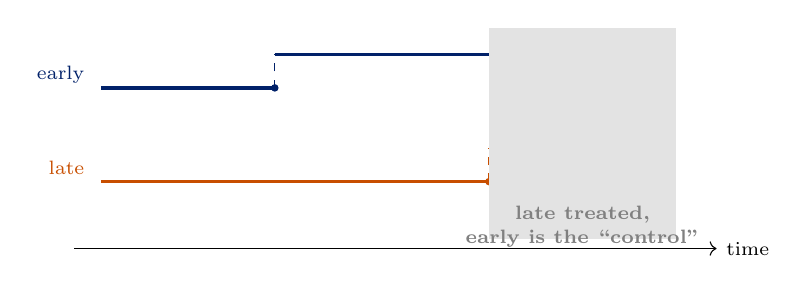
\begin{tikzpicture}[scale=0.85]
  \draw[->] (0,0) -- (9.6,0) node[right]{\scriptsize time};
  % early unit
  \draw[dukeblue,very thick] (0.4,2.4) -- (3.0,2.4);
  \draw[dukeblue,very thick] (3.0,2.9) -- (9.0,2.9);
  \draw[dukeblue,dashed] (3.0,2.4) -- (3.0,2.9);
  \node[dukeblue,left] at (0.3,2.6) {\scriptsize early};
  \fill[dukeblue] (3.0,2.4) circle (1.6pt);
  % late unit
  \draw[accent,very thick] (0.4,1.0) -- (6.2,1.0);
  \draw[accent,very thick] (6.2,1.5) -- (9.0,1.5);
  \draw[accent,dashed] (6.2,1.0) -- (6.2,1.5);
  \node[accent,left] at (0.3,1.2) {\scriptsize late};
  \fill[accent] (6.2,1.0) circle (1.6pt);
  % shaded window
  \fill[gray!22] (6.2,0.15) rectangle (9.0,3.3);
  \node[gray] at (7.6,0.5) {\scriptsize \textbf{late treated,}};
  \node[gray] at (7.6,0.15) {\scriptsize \textbf{early is the ``control''}};
\end{tikzpicture}
\end{center}
\vskip-4pt
\begin{itemize}\itemsep2pt
  \item In the shaded window, TWFE uses the \emph{early-treated} unit as a control
        for the late-treated one.
  \item If the early unit's effect is still evolving, that evolution is subtracted
        from the late unit's effect, and enters with a \alert{negative weight}.
  \item With dynamic effects, TWFE can be the wrong \emph{sign} even when every
        unit-level effect is positive.
\end{itemize}
\end{frame}


\begin{frame}[allowframebreaks,t]{The Forbidden Comparison, in Algebra\core}
Take the late-versus-early $2\times2$ from the shaded window: late switches from
untreated to treated, early is \emph{treated throughout}. Suppose parallel
trends holds exactly and untreated outcomes are flat, so every change in $Y$ is
a treatment effect. Then
\begin{align*}
  \hat\beta^{2\times2}_{\text{late vs.\ early}}
  = \underbrace{\text{ATT}_{\text{late}}(\text{post})}_{\text{what we want}}
  \;-\; \underbrace{\Big[\text{ATT}_{\text{early}}(\text{post}) - \text{ATT}_{\text{early}}(\text{pre})\Big]}_{\alert{\text{the \emph{growth} in early's effect over the window}}} .
\end{align*}
\vskip2pt
With numbers; no noise, no trends, every true effect positive:
\begin{center}\small
\renewcommand{\arraystretch}{1.2}
\begin{tabular}{lccc}
\toprule
 & $t=3$ & $t=4$ & Change \\
\midrule
Late (treated at $t{=}4$; effect $1$) & $0$ & $1$ & $+1$ \\
Early (treated at $t{=}2$; effects $1,2,3$) & $2$ & $3$ & $+1$ \\
\midrule
 & & & $\hat\beta^{2\times2} = 0$ \\
\bottomrule
\end{tabular}
\end{center}
\vskip3pt
\begin{itemize}\itemsep2pt
  \item Late's true effect is $+1$; this comparison returns $0$. If early's
        effect grew by $2$ per period instead, it would return $\alert{-1}$.
  \item If effects were constant ($1,1,1$), the bracketed term would vanish and
        the comparison would be harmless, which is exactly why the problem
        stayed invisible for thirty years of constant-effect thinking.
\end{itemize}
\end{frame}

\begin{frame}{The Goodman-Bacon Decomposition\adv}
With staggered timing, the TWFE estimate is a weighted average of every possible
$2\times2$ comparison in the data:
\begin{align*}
  \hat\beta^{\text{TWFE}} = \sum_{\text{pairs}} s_{ab}\;\hat\beta^{2\times2}_{ab} ,
  \qquad \sum s_{ab} = 1 ,
\end{align*}
where the weights $s_{ab}$ depend on group sizes and on the \emph{variance of
treatment} within each pair, largest for pairs whose treatment switches
mid-window. (The next frame writes them out.)
\vskip3pt
Three kinds of comparison arise:
\begin{enumerate}\itemsep1pt
  \item Treated versus \textbf{never-treated}, clean.
  \item \textbf{Earlier} treated versus \textbf{later} treated, before the later
        group switches, clean.
  \item \alert{\textbf{Later} treated versus \textbf{earlier} treated, after the
        earlier group switches, the forbidden comparison.}
\end{enumerate}
\vskip3pt
Type 3 uses already-treated units as controls. If their effects are still
evolving, that evolution is subtracted from the late group's effect.
\end{frame}

\begin{frame}[allowframebreaks,t]{The Goodman-Bacon Weights, Explicitly\adv}
Let $n_k, n_l, n_U$ be the groups' sample shares and $\bar D_j$ the fraction of
the panel that group $j$ spends treated ($k$ treated earlier than $l$). Up to a
common normalization, the weight on each $2\times2$ is the product of the pair's
group sizes and the \emph{variance of the treatment dummy within that pair's
window}:
\begin{align*}
  s_{kU} &\propto n_k\, n_U\;\bar D_k\big(1-\bar D_k\big)
  && \text{treated vs.\ never-treated} \\[2pt]
  s^{\,k}_{kl} &\propto n_k\, n_l\;\big(\bar D_k - \bar D_l\big)\big(1-\bar D_k\big)
  && \text{early vs.\ late, before late switches} \\[2pt]
  s^{\,l}_{kl} &\propto n_k\, n_l\;\bar D_l\big(\bar D_k-\bar D_l\big)
  && \alert{\text{late vs.\ early, after early switches}}
\end{align*}
\vskip2pt
\begin{itemize}\itemsep3pt
  \item Every weight has the $\bar D(1-\bar D)$ shape of a Bernoulli variance,
        so \alert{groups treated near the middle of the panel dominate}: the
        weights come from OLS mechanics, not from group sizes alone and not from
        any estimand you chose. Compare Week 1's variance-weighting result: same
        phenomenon, new costume.
  \item The forbidden weight $s^{\,l}_{kl}$ is not negligible in general: it
        grows with $\bar D_k$, i.e.\ with how long the early group has already
        been treated when the late group switches.
  \item All of this is computable from the data alone:
        \texttt{bacondecomp::bacon()} lists every $2\times2$, its estimate, and
        its weight. We decompose a real TWFE estimate in lab.
\end{itemize}
\end{frame}

\begin{frame}[allowframebreaks,t]{Where the Negative Weights Come From\adv}
FWL (Week 1) reduces TWFE to a bivariate regression on the
\emph{double-demeaned} treatment. With $\bar D_i$, $\bar D_t$, $\bar D$ the
unit, period, and grand means of $D_{it}$:
\begin{align*}
  \hat\beta^{\text{TWFE}}
  = \frac{\sum_{it} \tilde D_{it}\, Y_{it}}{\sum_{it} \tilde D_{it}^2},
  \qquad
  \tilde D_{it} = D_{it} - \bar D_i - \bar D_t + \bar D .
\end{align*}
Substitute $Y_{it} = \alpha_i + \lambda_t + \tau_{it} D_{it} + \epsilon_{it}$:
the fixed effects are annihilated because $\tilde D$ has zero unit and period
sums, and $\sum_{it}\tilde D_{it}^2 = \sum_{(i,t):D_{it}=1}\tilde D_{it}$, so
\begin{align*}
  \plim\,\hat\beta^{\text{TWFE}}
  = \sum_{(i,t):\,D_{it}=1} w_{it}\,\tau_{it},
  \qquad
  w_{it} = \frac{\tilde D_{it}}{\sum_{(i,t):\,D_{it}=1}\tilde D_{it}},
  \qquad \sum w_{it} = 1 .
\end{align*}
\vskip2pt
\begin{itemize}\itemsep3pt
  \item For a \emph{treated} cell, $\tilde D_{it} = 1 - \bar D_i - \bar D_t + \bar D$,
        which is \alert{negative exactly when $\bar D_i + \bar D_t > 1 + \bar D$}:
        a unit treated for most of the panel, observed in a period when most of
        the sample is treated. That is the early adopter, late in the panel.
  \item Intuition: OLS rewards cells whose treatment status is
        \emph{surprising} given their unit and period averages. An early
        adopter's late-period treatment is completely unsurprising, so its
        effect is priced at zero, or below zero.
  \item The weights are a mechanical fact about OLS and are there even under
        constant effects, harmlessly. Heterogeneous $\tau_{it}$ is what turns
        strange weights into a wrong answer.
\end{itemize}
\end{frame}

\begin{frame}[allowframebreaks,t]{Negative Weights: Consequences and Diagnostics\adv}
\srct{de Chaisemartin and D'Haultf\oe uille (2020)} generalize the previous
frame's calculation, allowing covariates and non-binary treatments, and show
that negative weights are the rule in staggered designs, not a corner case.
\vskip3pt
\begin{itemize}\itemsep3pt
  \item Consequence: TWFE can have the \alert{wrong sign} even when every
        $\tau_{it} > 0$. This is not a small-sample problem; it survives
        $n\to\infty$, because the weights, not the noise, are at fault.
  \item By the formula, the negative weights fall on units treated \emph{early}
        and observed over a \emph{long} post-period, exactly the units carrying
        the most information about long-run effects. TWFE quietly discounts, and
        then inverts, the long run.
  \item \textbf{Diagnostic}: compute the weights
        (\texttt{TwoWayFEWeights::twowayfeweights}) and report how many are
        negative and what share of the total mass they carry. Small negative
        mass is reassuring about \emph{this particular} problem; it says nothing
        about parallel trends or about dynamic-effect contamination, so it is
        one diagnostic, not a validity test.
  \item \srct{Sun and Abraham (2021)} show the same contamination in event-study
        coefficients: with staggered timing, the TWFE $\hat\tau_k$ at lag $k$ is
        a weighted combination of \emph{every} cohort's effects at \emph{every}
        lag, with weights that need not be positive or sum to one lag by lag. So
        apparent pre-trends can be artefacts of post-treatment dynamics, and a
        clean pre-trend plot from raw TWFE proves nothing.
\end{itemize}
\vskip3pt
\alert{TWFE is fine when treatment timing is common, or when effects are
genuinely constant.} It is unreliable exactly where sociologists use it most.
\end{frame}

\begin{frame}[allowframebreaks,t]{Callaway--Sant'Anna: Build Clean Blocks, Then Aggregate}
Define the \alert{group-time average treatment effect} for cohort $g$ at time $t$:
\begin{align*}
  ATT(g,t) = \E\big[Y_t(g) - Y_t(\infty) \mid G_i = g\big] ,
\end{align*}
identified by comparing cohort $g$ to units \emph{not yet treated} at $t$ (or to
never-treated units), using only periods before $g$ as the baseline. Under
cohort-level parallel trends and no anticipation,
\begin{align*}
  ATT(g,t) = \E\big[Y_{t} - Y_{g-1} \mid G_i = g\big]
           - \E\big[Y_{t} - Y_{g-1} \mid \text{not yet treated at } t\big] :
\end{align*}
a clean $2\times2$. The baseline $g-1$ predates cohort $g$'s treatment, the
comparison group has not started treatment by $t$, and no already-treated unit
is ever used as a control.
\vskip3pt
\begin{itemize}\itemsep2pt
  \item Under \emph{conditional} parallel trends, each block can be estimated by
        IPW, outcome regression, or a doubly robust estimator, \alert{Week 6,
        reappearing inside a DID}.
  \item \textbf{Then choose an aggregation}, and the choice is an estimand choice:
  \begin{itemize}\itemsep1pt
    \item \emph{simple}: average over all treated $(g,t)$;
    \item \emph{dynamic}: average by $t-g$, giving an event-study path;
    \item \emph{group}: average within cohort, showing who benefited;
    \item \emph{calendar}: average within period, showing when.
  \end{itemize}
  \item Sun--Abraham reaches the same place through an interaction-weighted
        regression; Borusyak--Jaravel--Spiess by imputing $Y(0)$ from untreated
        cells.
\end{itemize}
\end{frame}


\begin{frame}{The Modern Estimators\core}
All of them share one principle: \alert{never use an already-treated unit as a
control}. Build clean $2\times 2$ comparisons, then aggregate with weights you
choose.
\vskip3pt
\begin{center}\footnotesize
\renewcommand{\arraystretch}{1.35}
\begin{tabular}{lll}
\toprule
Method & Idea & \texttt{R} \\
\midrule
Callaway--Sant'Anna (2021) & group-time ATT$(g,t)$, never- or
  not-yet-treated controls & \texttt{did} \\
Sun--Abraham (2021) & interaction-weighted event study & \texttt{fixest::sunab} \\
de Chaisemartin--D'Haultf\oe uille & clean comparisons at switch dates &
  \texttt{DIDmultiplegt} \\
Borusyak--Jaravel--Spiess & impute $Y(0)$ from untreated cells &
  \texttt{didimputation} \\
Stacked / cohort DID & one clean event window per cohort & manual \\
\bottomrule
\end{tabular}
\end{center}
\vskip4pt
Callaway--Sant'Anna also allows \textbf{conditional} parallel trends: trends
parallel only after adjusting for covariates, estimated by IPW, regression, or
doubly robust, Week 6, reappearing.
\end{frame}

\begin{frame}[allowframebreaks,t]{Honest Inference About Pre-Trends}
Rather than testing pre-trends and proceeding as if they had passed,
\srct{Rambachan and Roth (2023)} propose bounding how badly parallel trends could
fail.
\vskip4pt
\begin{itemize}\itemsep3pt
  \item Their ``relative magnitudes'' restriction bounds how much the
        \emph{change} in the trend violation after treatment can exceed the
        largest change observed before it, by a factor $\bar M$, and the
        resulting confidence sets account for sampling uncertainty in the
        pre-period estimates rather than treating them as known.
  \item Report the \emph{breakdown value}: how large $\bar M$ would have to be
        before your conclusion reverses.
  \item This turns an untestable assumption into a quantitative claim, exactly
        the move sensitivity analysis made in Week 6.
  \item \texttt{HonestDiD}.
\end{itemize}
\vskip3pt
\begin{alertblock}{Inference reminder}
\srct{Bertrand, Duflo, and Mullainathan (2004)}: cluster on the unit at which
treatment varies. With few clusters, use CR2 or a wild cluster bootstrap
(Week 2).
\end{alertblock}
\end{frame}

\begin{frame}{A DID Checklist\core}
\begin{enumerate}\itemsep2pt
  \item State the estimand: ATT for whom, over which post-treatment window?
  \item Plot the raw group means over time. Before any regression.
  \item Is timing staggered? If so, \alert{do not use plain TWFE}. Use a modern
        estimator, and report the TWFE estimate only for comparison.
  \item Report an event-study plot with pre-period coefficients, using
        Sun--Abraham or Callaway--Sant'Anna rather than raw TWFE leads.
  \item Justify the scale (levels or logs) on substantive grounds.
  \item Cluster on the treatment-assignment unit; report the number of clusters.
  \item Report a sensitivity analysis for parallel trends.
  \item Placebo: a pre-treatment outcome, or an untreated outcome that the policy
        should not affect.
\end{enumerate}
\end{frame}

\begin{frame}{Looking Ahead}
\begin{itemize}\itemsep4pt
  \item Fixed effects difference away time-invariant confounders, a real gain,
        bought with precision and with a new assumption about trends.
  \item The staggered-adoption literature is a case study in how a method can be
        standard for decades and still be wrong. Read papers published before
        2021 with this in mind, including your own field's classics.
  \item \textbf{Next week}: what to do when there is only \emph{one} treated
        unit, and ``the control group'' has to be constructed.
  \item Notice that conditional parallel trends brought Week 6 back inside a
        DID: once trends are only parallel given covariates, you need a weighting
        or outcome model again, and all of Week 6's cautions return with it.
\end{itemize}
\vskip4pt
\begin{block}{Problem Set 4}
Assigned today, due Monday November 9. Covers Weeks 7 and 9.
\end{block}
\end{frame}


\begin{frame}[allowframebreaks,t]{References}
\footnotesize
\begin{itemize}\itemsep3pt
\item Angrist, Joshua D. and J\"orn-Steffen Pischke. 2009.
\textit{Mostly Harmless Econometrics}. Princeton University Press. [Ch.\ 5]
\item Bertrand, Marianne, Esther Duflo, and Sendhil Mullainathan. 2004. ``How
Much Should We Trust Differences-in-Differences Estimates?''
\textit{Quarterly Journal of Economics} 119(1): 249--275.
\item Borusyak, Kirill, Xavier Jaravel, and Jann Spiess. 2024. ``Revisiting
Event-Study Designs: Robust and Efficient Estimation.''
\textit{Review of Economic Studies} 91(6): 3253--3285.
\item Callaway, Brantly and Pedro H.C. Sant'Anna. 2021. ``Difference-in-Differences
with Multiple Time Periods.'' \textit{Journal of Econometrics} 225(2): 200--230.
\item de Chaisemartin, Cl\'ement and Xavier D'Haultf\oe uille. 2020. ``Two-Way
Fixed Effects Estimators with Heterogeneous Treatment Effects.''
\textit{American Economic Review} 110(9): 2964--2996.
\item Goodman-Bacon, Andrew. 2021. ``Difference-in-Differences with Variation in
Treatment Timing.'' \textit{Journal of Econometrics} 225(2): 254--277.
\item Rambachan, Ashesh and Jonathan Roth. 2023. ``A More Credible Approach to
Parallel Trends.'' \textit{Review of Economic Studies} 90(5): 2555--2591.
\item Roth, Jonathan. 2022. ``Pretest with Caution: Event-Study Estimates after
Testing for Parallel Trends.'' \textit{American Economic Review: Insights} 4(3):
305--322.
\item Roth, Jonathan, Pedro H.C. Sant'Anna, Alyssa Bilinski, and John Poe. 2023.
``What's Trending in Difference-in-Differences?''
\textit{Journal of Econometrics} 235(2): 2218--2244.
\item Sun, Liyang and Sarah Abraham. 2021. ``Estimating Dynamic Treatment Effects
in Event Studies with Heterogeneous Treatment Effects.''
\textit{Journal of Econometrics} 225(2): 175--199.
\end{itemize}
\end{frame}

\end{document}
